%%% -*- TeX-master: "case-study.tex" -*-
\section{The minmod limiter}
\label{sec:minmod}

Simulation of physical phenomena is an important use case for differential equation solvers, consequently ways to reduce or eliminate numerical errors have always been of interest.
One of the first ideas was researched by van Leer in 1979, when he proposed the $\minmod$ limiter\cite{VanLeer1979}.
A limiter in general restricts the steepness of the gradient of $U$ to sensible values where the bounds may be computed based on the current state or even set based on domain knowledge.
Of interest for us is in particular the former type because of its wide applicability.

The idea behind $\minmod$ specifically is to prevent the accidental introduction of new extrema into $U$.
It was originally defined for the case that the solution on cell $i$ is approximated by a first-order polynomial $c_{i}^{1}x + c_{i}^{0}$.
The limiter then updates all the slopes $c_{i}^{1}$ to $\tilde{c}_{i}^{1}$ by
\begin{equation*}
  \tilde{c}_{i}^{1} = \minmod\left( c_{i}^{1}, \frac{c_{i + 1}^{0} - c_{i}^{0}}{\Delta x}, \frac{c_{i}^{0} - c_{i - 1}^{0}}{\Delta x} \right)
\end{equation*}
where the $\minmod$ operation is defined by
\begin{equation*}
  \minmod(a, b, c) = \begin{cases}
    \displaystyle\argmin_{x \in \{ a, b, c \}} |x| & \text{if} \sgn(a) = \sgn(b) = \sgn(c)\\
    0 & \text{otherwise}
  \end{cases}
\end{equation*}
So the slope on each cell is bounded by the forward and backward difference quotients of the cell and its neighbor's average values that approach the true first derivative as $\Delta x$ goes to $0$.

The effect of this limiter is demonstrated in Figure \ref{fig:minmod}.
In Figure \ref{fig:minmod-steep} the slope is limited so that the values do not exceed the average levels on neighboring cells.
Figure \ref{fig:minmod-extremum} shows how the approximation is reduced to first order in the case of an extremum as well as in the case that the slope does not agree with the trend set by the cell's neighbors (Figure \ref{fig:minmod-trend}).
\begin{figure*}
  \centering
  \begin{subfigure}{0.27\textwidth}
    \centering
    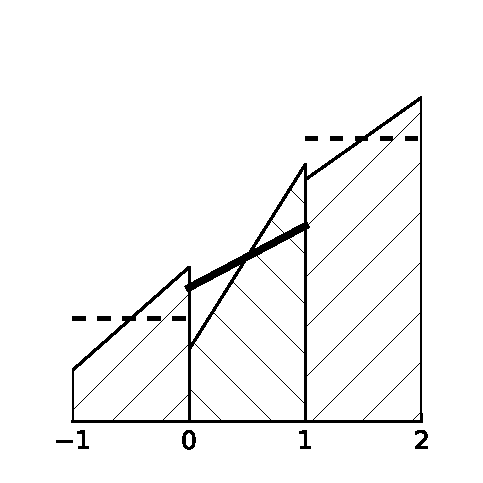
\includegraphics[width=\textwidth]{figures/minmod-a}
    \caption{Too steep}
    \label{fig:minmod-steep}
  \end{subfigure}
  \hfill
  \begin{subfigure}{0.27\textwidth}
    \centering
    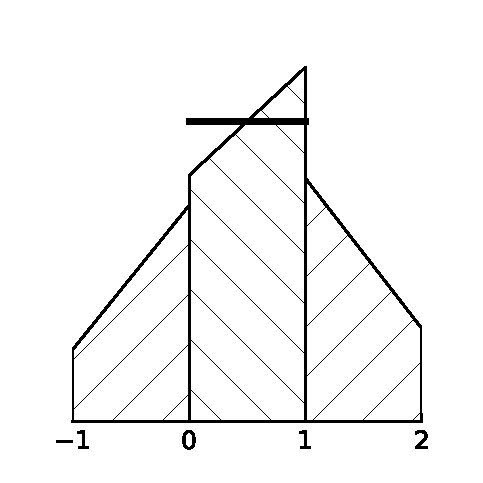
\includegraphics[width=\textwidth]{figures/minmod-b}
    \caption{Extremum in cell}
    \label{fig:minmod-extremum}
  \end{subfigure}
  \hfill
  \begin{subfigure}{0.27\textwidth}
    \centering
    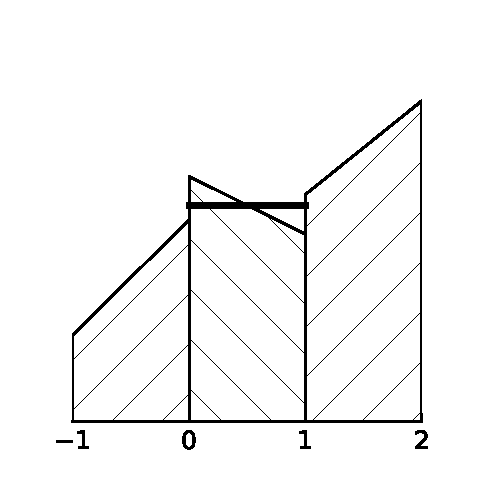
\includegraphics[width=\textwidth]{figures/minmod-c}
    \caption{Trend disagreement}
    \label{fig:minmod-trend}
  \end{subfigure}
  \caption{Three cell domain showcasing when the minmod limiter becomes active. Dashed lines indicate average levels in a cell, bold lines designate limited slopes. Figure modeled after \cite[Figure 3]{VanLeer1979}.}
  \label{fig:minmod}
\end{figure*}

To see how such a scheme prevents the formation of new extrema, consider again Figure \ref{fig:minmod-steep}.
Before the limiter application the polynomial approximation of the center cell introduced new extrema at both of the cell's boundary points.
Afterwards the right boundary is fixed but the interesting case occurs on the left-hand side.
Here the extremum persists through the limiting of the center cell.
However, it will be fixed as well when the leftmost cell is limited because the new slope of the center cell will also be an upper bound for the slope on the left-hand cell since one cell's backward difference quotient is its neighbor's forward difference quotient.
So in the extreme case the slopes on neighboring cells can be at most as steep as the line that passes through both cells' center points.
The argument for the way Figures \ref{fig:minmod-extremum} and \ref{fig:minmod-trend} were limited require arguments from Section \ref{sec:total-variation} and will be discussed at the end of it.
